\section{Faulted 3-phase network (1)}
\subsection{Circuit diagram}
\begin{figure}[H]
    \centering
    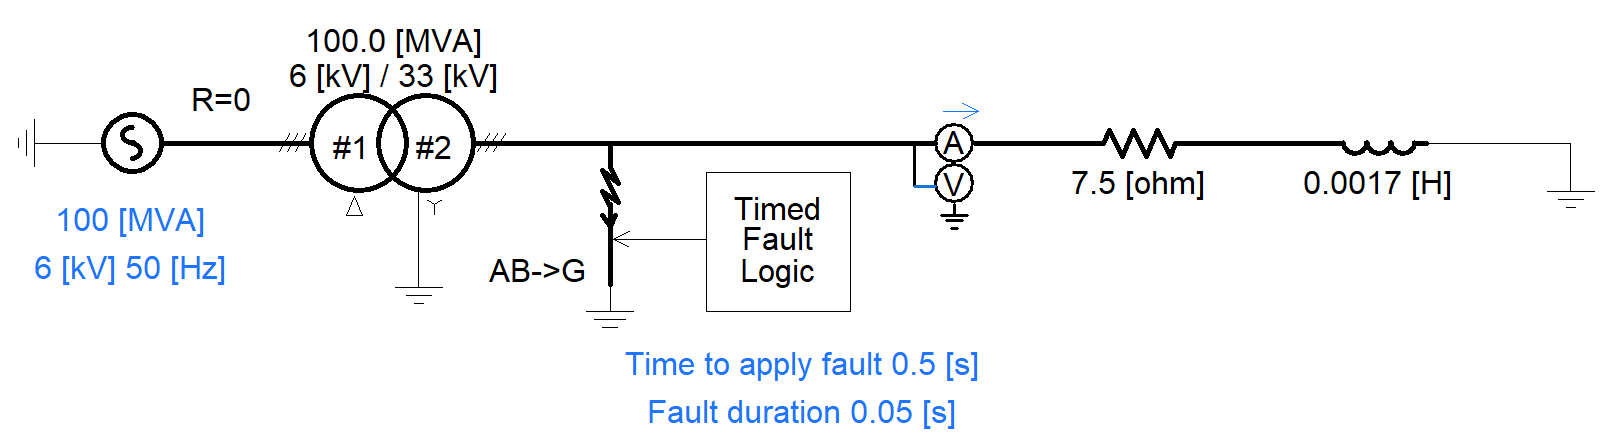
\includegraphics[width = \textwidth]{img/figure12.png}
    \caption{Circuit diagram to show distribution network.}
    \label{fig:distributionNetwork}
\end{figure}
\subsection{Voltage and current waveforms}
\begin{figure}[H]
    \centering
    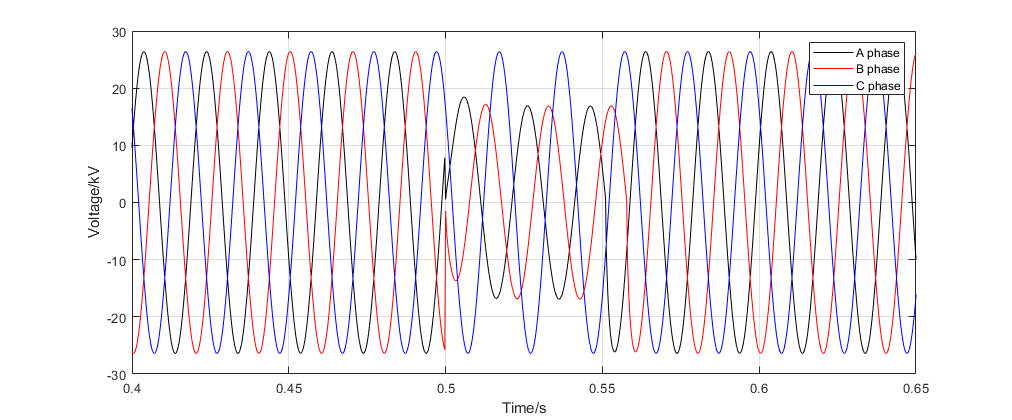
\includegraphics[width = \textwidth]{img/figure14.png}
    \caption{Faulted phase voltages over time from \SI{0.4}{\second} to \SI{0.65}{\second}.}
    \label{fig:fault1}
\end{figure}
\begin{figure}[H]
    \centering
    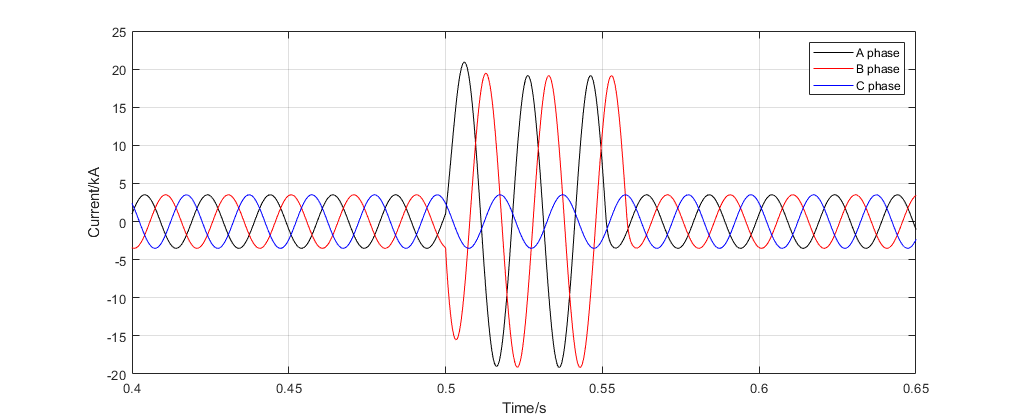
\includegraphics[width = \textwidth]{img/figure13.png}
    \caption{Faulted phase currents over time from \SI{0.4}{\second} to \SI{0.65}{\second}.}
    \label{fig:fault2}
\end{figure}
\subsection{Discussion}
From Figure \ref{fig:fault1}, a collapse in the voltages of the faulted phases (A and B) is observed. There is no significant effect on the voltage of phase C. Phase angle is disrupted; phase A and C are \SI{180}{\degree} out of phase with respect to one another during the fault, whilst phase B is \SI{120}{\degree} out of phase with respect to phase A.

From Figure \ref{fig:fault2}, the faulted phases see a considerable increase in current magnitude due to the sudden increase in ground current flow. However, all phases remain at \SI{120}{\degree} phase angle with respect to the other phases. Unfaulted phase remains unaffected.